% # 6.2 基于锁的并发数据结构

基于锁的并发数据结构需要确保访问线程持有锁的时间最短,对于只有一个互斥量的数据结构来说十分困难。需要锁之外的操作不能访问数据,保证不会产生条件竞争。使用多个互斥量保护数据结构不同的区域时,问题会更加明显。当操作需要获取多个互斥锁时,可能会产生死锁,所以使用多个互斥量时要格外小心。

本节将使用6.1.1节的指导建议,来设计简单的数据结构——使用互斥量和锁的来保护数据。每个例子都在保证是线程安全的前提下,对数据结构并发访问的概率(机会)进行提高。

先来看看第3章中栈的实现,只使用了一个互斥量。但这个结构线程安全吗?它离真正的并发访问还差什么呢?

\mySubsubsection{6.2.1}{线程安全栈——使用锁}

先把第3章中线程安全的栈拿过来看看:(试图实现一个线程安全版的\texttt{std:stack<>})

代码6.1 线程安全栈的类定义

\begin{cpp}
#include <exception>

struct empty_stack: std::exception
{
  const char* what() const throw();
};

template<typename T>
class threadsafe_stack
{
private:
  std::stack<T> data;
  mutable std::mutex m;
public:
  threadsafe_stack(){}
  threadsafe_stack(const threadsafe_stack& other)
  {
    std::lock_guard<std::mutex> lock(other.m);
    data=other.data;
  }

  threadsafe_stack& operator=(const threadsafe_stack&) = delete;

  void push(T new_value)
  {
    std::lock_guard<std::mutex> lock(m);
    data.push(std::move(new_value));  // 1
  }
  std::shared_ptr<T> pop()
  {
    std::lock_guard<std::mutex> lock(m);
    if(data.empty()) throw empty_stack();  // 2
    std::shared_ptr<T> const res(
      std::make_shared<T>(std::move(data.top())));  // 3
    data.pop();  // 4
    return res;
  }
  void pop(T& value)
  {
    std::lock_guard<std::mutex> lock(m);
    if(data.empty()) throw empty_stack();
    value=std::move(data.top());  // 5
    data.pop();  // 6
  }
  bool empty() const
  {
    std::lock_guard<std::mutex> lock(m);
    return data.empty();
  }
};
\end{cpp}

首先,互斥量m可保证线程安全,对每个成员函数进行加锁保护。保证在同一时间内,只有一个线程可以访问到数据。

其次,empty()和pop()之间会存在竞争,代码会在pop()上锁时,显式的查询栈是否为空,所以不是恶性竞争。pop()直接返回弹出值,就可避免\texttt{std::stack<>}中top()和pop()之间的竞争。

再次,类中也有一些异常源。因为上锁操作是每个成员函数所做的第一个操作,所以对互斥量上锁可能会抛出异常。因无数据修改,所以安全。解锁互斥量不会失败,所以这段代码很安全,并且使用\texttt{std::lock\_guard<>}也能保证互斥量上锁的状态。

对data.push()①的调用可能会抛出一个异常,不是拷贝/移动数据,就是内存不足。不管哪种情况,\texttt{std::stack<>}都能保证其安全性,所以也没有问题。

pop()第一个重载中,代码可能会抛出empty\_stack异常②,数据没有修改,是安全的。创建res③时,也可能会抛出异常,两个原因:\texttt{std::make\_shared}无法分配出足够的内存去创建新对象,并且内部数据需要引用新对象;或者在拷贝或移动构造到新分配的内存中时抛出异常。两种情况下,C++运行时库和标准库能确保不会出现内存泄露,并且新创建的对象(如果有的话)都能正确销毁。因为没有对栈进行任何修改,所以没问题。当调用data.pop()④时,能保证不抛出异常并返回结果,所以这个重载的pop()是“异常-安全”的。

第二个重载pop()除了在拷贝赋值或移动赋值时会抛出异常⑤,当构造新对象和\texttt{std::shared\_ptr}实例时都不会抛出异常。同样,调用data.pop()⑥(这个成员函数保证不会抛出异常)之前,没有对数据结构进行修改,所以这个函数也是“异常-安全”的。

最后,empty()不会修改任何数据,所以也是“异常-安全”函数。

当调用持有一个锁的用户代码时,有两个地方可能会死锁:拷贝构造或移动构造(①,③)和拷贝赋值或移动赋值操作⑤。还有一个潜在死锁的地方位于用户定义的new操作符。无论是直接调用栈的成员函数的方式,还是在成员函数进行操作时,对已插入或删除的数据进行操作的方式对锁进行获取,都可能造成死锁。不过,用户要对栈负责,当栈未对数据进行拷贝或分配时,用户就不能随意的将其添加到栈中。

所有成员函数都使用\texttt{std::lock\_guard<>}保护数据,所以栈成员函数才是“线程安全”的。当然,构造与析构函数不是“线程安全”的,但构造与析构只有一次。调用不完全构造对象或是已销毁对象的成员函数,无论在哪种编程方式下都不可取。所以,用户就要保证在栈对象完成构建前,其他线程无法对其进行访问。并且,要保证在栈对象销毁后,停止所有线程的访问操作。

即使在多线程下,并发调用成员函数也是安全的(因为使用锁)。同时,要保证在单线程的情况下,数据结构能做出正确反应。串行化线程会隐性的限制程序性能,这就是栈争议最大的地方:当一个线程在等待锁时,就会无所事事。对于栈来说,等待添加元素是没有意义的,所以当线程需要等待时,会定期检查empty()或pop(),以及对empty\_stack异常进行关注。这样的现实会限制栈的实现方式,线程等待时会浪费宝贵的资源去检查数据,或要求用户编写等待和提示的代码(例如:使用条件变量),这就使内部锁失去存在的意义,也造成资源的浪费。

第4章中的队列就是使用条件内部变量进行等待的数据结构,接下来我们就来了解一下。

\mySubsubsection{6.2.2}{线程安全队列——使用锁和条件变量}

代码6.2中重新实现了第4章中的线程安全队列,与使用仿\texttt{std::stack<>}建立的栈类似,队列也参照了\texttt{std::queue<>}。不过,与标准容器的接口不同,我们要设计的是线程安全的数据结构。

代码6.2 使用条件变量实现的线程安全队列

\begin{cpp}
template<typename T>
class threadsafe_queue
{
private:
  mutable std::mutex mut;
  std::queue<T> data_queue;
  std::condition_variable data_cond;

public:
  threadsafe_queue()
  {}

  void push(T data)
  {
    std::lock_guard<std::mutex> lk(mut);
    data_queue.push(std::move(data));
    data_cond.notify_one();  // 1
  }

  void wait_and_pop(T& value)  // 2
  {
    std::unique_lock<std::mutex> lk(mut);
    data_cond.wait(lk,[this]{return !data_queue.empty();});
    value=std::move(data_queue.front());
    data_queue.pop();
  }

  std::shared_ptr<T> wait_and_pop()  // 3
  {
    std::unique_lock<std::mutex> lk(mut);
    data_cond.wait(lk,[this]{return !data_queue.empty();});  // 4
    std::shared_ptr<T> res(
      std::make_shared<T>(std::move(data_queue.front())));
    data_queue.pop();
    return res;
  }

  bool try_pop(T& value)
  {
    std::lock_guard<std::mutex> lk(mut);
    if(data_queue.empty())
      return false;
    value=std::move(data_queue.front());
    data_queue.pop();
    return true;
  }

  std::shared_ptr<T> try_pop()
  {
    std::lock_guard<std::mutex> lk(mut);
    if(data_queue.empty())
      return std::shared_ptr<T>();  // 5
    std::shared_ptr<T> res(
      std::make_shared<T>(std::move(data_queue.front())));
    data_queue.pop();
    return res;
  }

  bool empty() const
  {
    std::lock_guard<std::mutex> lk(mut);
    return data_queue.empty();
  }
};
\end{cpp}

除了在push()①中调用data\_cond.notify\_one(),以及wait\_and\_pop()②③,6.2中对队列的实现与6.1中对栈的实现类似。两个重载的try\_pop()除了在队列为空时抛出异常,其他的与6.1中pop()函数完全一样。不同的是,6.1中对值的检索会返回一个bool值,而6.2中当指针指向空值的时返回NULL⑤,这也是实现栈的一个有效方式。所以,即使排除掉wait\_and\_pop()函数,之前对栈的分析依旧适用于这里。

wiat\_and\_pop()函数是等待队列向栈进行输入的一个解决方案。比起持续调用empty(),等待线程调用wait\_and\_pop()函数和条件变量的方式要好很多。对于data\_cond.wait()的调用,直到队列中有元素的时候才会返回,所以不用担心会出现一个空队列的情况,且互斥锁会保护数据。因为不变量并未发生变化,所以函数不会增加新的条件竞争或死锁的可能。

异常安全会有一些变化,不止一个线程等待对队列进行推送操作时,只会有一个线程因data\_cond.notify\_one()而继续工作。但是,如果工作线程在wait\_and\_pop()中抛出一个异常,例如:构造新的\texttt{std::shared\_ptr<>}对象④时抛出异常,那么其他线程则会永世长眠。这种情况不可以,所以调用函数需要改成data\_cond.notify\_all(),这个函数将唤醒所有的工作线程,不过当大多线程发现队列依旧是空时,又会耗费资源让线程重新进入睡眠。第二种替代方案,有异常抛出时,让wait\_and\_pop()函数调用notify\_one(),从而让个另一个线程去索引存储的值。第三种替代方案,将\texttt{std::shared\_ptr<>}的初始化过程移到push()中,并且存储\texttt{std::shared\_ptr<>}实例,而不是直接使用数据值,将\texttt{std::shared\_ptr<>}拷贝到内部\texttt{std::queue<>}中就不会抛出异常了,这样wait\_and\_pop()又是安全的了。下面的代码,就是根据第三种方案修改的。

代码6.3 持有\texttt{std::shared\_ptr<>}实例的线程安全队列

\begin{cpp}
template<typename T>
class threadsafe_queue
{
private:
  mutable std::mutex mut;
  std::queue<std::shared_ptr<T> > data_queue;
  std::condition_variable data_cond;
public:
  threadsafe_queue()
  {}

  void wait_and_pop(T& value)
  {
    std::unique_lock<std::mutex> lk(mut);
    data_cond.wait(lk,[this]{return !data_queue.empty();});
    value=std::move(*data_queue.front());  // 1
    data_queue.pop();
  }

  bool try_pop(T& value)
  {
    std::lock_guard<std::mutex> lk(mut);
    if(data_queue.empty())
      return false;
    value=std::move(*data_queue.front());  // 2
    data_queue.pop();
    return true;
  }

  std::shared_ptr<T> wait_and_pop()
  {
    std::unique_lock<std::mutex> lk(mut);
    data_cond.wait(lk,[this]{return !data_queue.empty();});
    std::shared_ptr<T> res=data_queue.front();  // 3
    data_queue.pop();
    return res;
  }

  std::shared_ptr<T> try_pop()
  {
    std::lock_guard<std::mutex> lk(mut);
    if(data_queue.empty())
      return std::shared_ptr<T>();
    std::shared_ptr<T> res=data_queue.front();  // 4
    data_queue.pop();
    return res;
  }

  void push(T new_value)
  {
    std::shared_ptr<T> data(
    std::make_shared<T>(std::move(new_value)));  // 5
    std::lock_guard<std::mutex> lk(mut);
    data_queue.push(data);
    data_cond.notify_one();
  }

  bool empty() const
  {
    std::lock_guard<std::mutex> lk(mut);
    return data_queue.empty();
  }
};
\end{cpp}

为让\texttt{std::shared\_ptr<>}持有数据的结果显而易见:pop()函数会持有一个变量的引用,为了接收这个新值,必须对存储的指针进行解引用①②。并且,返回调用函数前,pop()函数都会返回一个\texttt{std::shared\_ptr<>}实例,实例可以在队列中检索③④。

\texttt{std::shared\_ptr<>}持有数据的好处:新实例分配结束时,不会锁在push()⑤中(而在代码6.2中,只能在pop()持有锁时完成)。因为内存分配需要在性能上付出很高的代价(性能较低),因为减少了互斥量持有的时间,所以\texttt{std::shared\_ptr<>}对队列的性能有很大的提升,并且允许其他线程在分配内存的同时,可以对队列进行其他操作。

如同栈的例子一样,使用互斥量保护整个数据结构,不过会限制队列对并发的支持。虽然成员函数会阻塞多线程,但仍有一个线程能在任意时间内进行工作。不过,因为使用标准容器的原因,数据处于保护中(这种限制是实现中使用了\texttt{std::queue<>}),要对数据结构进行具体的控制,需要提供更多细粒度锁,来完成更高级的并发。

\mySubsubsection{6.2.3}{线程安全队列——使用细粒度锁和条件变量}

代码6.2和6.3中,使用一个互斥量对\textit{数据队列}(data\_queue)进行保护。为了使用细粒度锁,需要看一下队列内部的组成结构,并且将互斥量与每个数据相关联。

最简单的队列就是单链表了,如图6.1。队列里包含一个头指针,其指向链表中的第一个元素,并且每一个元素都会指向下一个元素。从队列中删除数据,其实就是将头指针指向下一个元素,并将之前头指针指向的值进行返回。

向队列中添加元素是要从结尾进行的。为了做到这点,队列里还有一个尾指针,其指向链表中的最后一个元素。新节点的加入将会改变尾指针的next指针,之前最后一个元素将会指向新添加进来的元素,新添加进来的元素的next将会使新的尾指针。当链表为空时,头/尾指针皆为NULL。

% ![](../../images/chapter6/6-1.png)
\begin{center}
    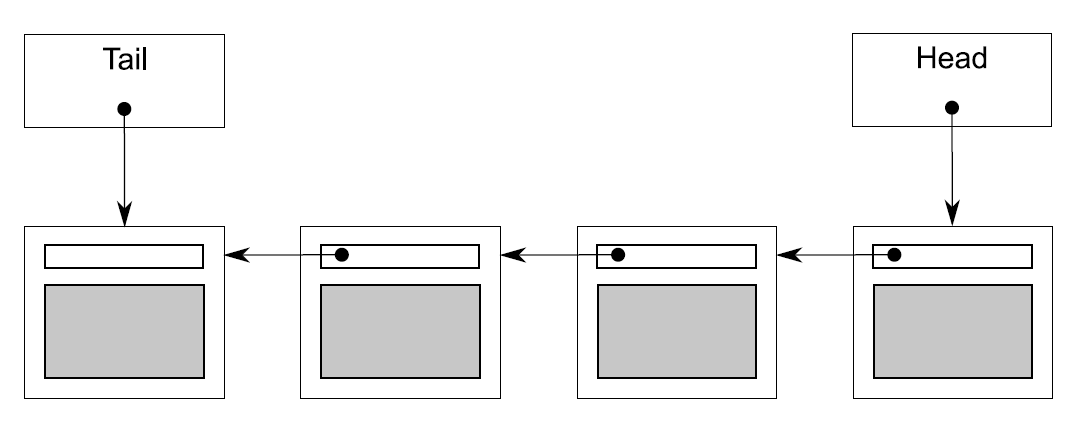
\includegraphics[width=0.7\textwidth]{content/chapter06/images/6-1.png}\\
    图6.1 用单链表表示的队列
\end{center}

下面的代码是一个简单队列的实现,基于代码6.2的精简版本。这个队列仅供单线程使用,所以实现中只有一个try\_pop()函数,没有wait\_and\_pop()函数。

代码6.4 队列实现——单线程版

\begin{cpp}
template<typename T>
class queue
{
private:
  struct node
  {
    T data;
    std::unique_ptr<node> next;

    node(T data_):
    data(std::move(data_))
    {}
  };

  std::unique_ptr<node> head;  // 1
  node* tail;  // 2

public:
  queue()
  {}
  queue(const queue& other)=delete;
  queue& operator=(const queue& other)=delete;
  std::shared_ptr<T> try_pop()
  {
    if(!head)
    {
      return std::shared_ptr<T>();
    }
    std::shared_ptr<T> const res(
      std::make_shared<T>(std::move(head->data)));
    std::unique_ptr<node> const old_head=std::move(head);
    head=std::move(old_head->next);  // 3
    return res;
  }

  void push(T new_value)
  {
    std::unique_ptr<node> p(new node(std::move(new_value)));
    node* const new_tail=p.get();
    if(tail)
    {
      tail->next=std::move(p);  // 4
    }
    else
    {
      head=std::move(p);  // 5
    }
    tail=new_tail;  // 6
  }
};
\end{cpp}

首先,代码6.4中使用了\texttt{std::unique\_ptr<node>}来管理节点,因为其能保证节点(其引用数据的值)在删除时候,不需要使用delete操作。这样的关系链表,管理着从头结点到尾节点的每一个原始指针,就需要\texttt{std::unique\_ptr<node>}类型的结点引用。

虽然,这种实现对于单线程来说没什么问题,但当在多线程下尝试使用细粒度锁时,就会出现问题。因为在给定的实现中有两个数据项(head①和tail②),即便是使用两个互斥量来保护头指针和尾指针,也会出现问题。

最明显的问题就是push()可以同时修改头指针⑤和尾指针⑥,所以push()函数会同时获取两个互斥量。虽然会将两个互斥量都上锁,但这还不算太糟糕。糟糕的是push()和pop()都能访问next指针指向的节点:push()可更新tail->next④,随后try\_pop()读取read->next③。当队列中只有一个元素时,head==tail,所以head->next和tail->next是同一个对象,并且这个对象需要保护。不过,“在同一个对象在未被head和tail同时访问时,push()和try\_pop()锁住的是同一个锁”就不对了。

\textbf{通过分离数据实现并发}

可以使用“预分配虚拟节点(无数据),确保这个节点永远在队列的最后,用来分离头尾指针能访问的节点”的办法。对于一个空队列来说,head和tail都属于虚拟指针,而非空指针。因为当队列为空时,try\_pop()不能访问head->next了。当添加一个节点入队列时(这时有真实节点了),head和tail现在指向不同的节点,所以就不会在head->next和tail->next上产生竞争。缺点是,必须额外添加一个间接层次的指针数据来做虚拟节点。

代码6.5 带有虚拟节点的队列

\begin{cpp}
template<typename T>
class queue
{
private:
  struct node
  {
    std::shared_ptr<T> data;  // 1
    std::unique_ptr<node> next;
  };

  std::unique_ptr<node> head;
  node* tail;

public:
  queue():
    head(new node),tail(head.get())  // 2
  {}
  queue(const queue& other)=delete;
  queue& operator=(const queue& other)=delete;

  std::shared_ptr<T> try_pop()
  {
    if(head.get()==tail)  // 3
    {
      return std::shared_ptr<T>();
    }
    std::shared_ptr<T> const res(head->data);  // 4
    std::unique_ptr<node> old_head=std::move(head);
    head=std::move(old_head->next);  // 5
    return res;  // 6
  }

  void push(T new_value)
  {
    std::shared_ptr<T> new_data(
      std::make_shared<T>(std::move(new_value)));  // 7
    std::unique_ptr<node> p(new node);  //8
    tail->data=new_data;  // 9
    node* const new_tail=p.get();
    tail->next=std::move(p);
    tail=new_tail;
  }
};
\end{cpp}

try\_pop()不需要太多的修改。首先,可以拿head和tail③进行比较,这就要比检查指针是否为空的好,因为虚拟节点意味着head不可能是空指针。head是一个\texttt{std::unique\_ptr<node>}对象,需要使用head.get()来做比较。其次,因为node现在存在数据指针中①,就可以对指针进行直接检索④,而非构造一个T类型的新实例。push()函数的改动最大:必须在堆上创建一个T类型的实例,并让其与\texttt{std::shared\_ptr<>}对象相关联⑦(节点使用\texttt{std::make\_shared}为了避免内存二次分配,避免增加引用次数)。创建的新节点就成为了虚拟节点,所以不需要为new\_value提供构造函数⑧。这里需要将new\_value的副本赋给之前的虚拟节点⑨。最终,为了让虚拟节点存在于队列中,需要使用构造函数来创建它②。

现在的push()只能访问tail,而不能访问head,try\_pop()可以访问head和tail,但是tail只需在最开始进行比较,所以所存在的时间很短。重大的提升在于虚拟节点意味着try\_pop()和push()不能对同一节点进行操作,所以不再需要互斥了。现在,只需要使用一个互斥量来保护head和tail就够了。那么,现在应该锁哪里?

为了最大程度的并发化,所以需要上锁的时间尽可能的少。push()很简单:互斥量需要对tail的访问上锁,就需要对每个新分配的节点上锁⑧,还有对当前尾节点进行赋值时⑨也需要上锁,锁需要持续到函数结束时才能解开。

try\_pop()就不简单了。首先,需要使用互斥量锁住head,一直到head弹出。实际上,互斥量决定了哪一个线程进行弹出操作。一旦改变head⑤,才能解锁互斥量。当返回结果时,互斥量就不需要上锁了⑥,这使得访问tail需要尾互斥量。因为,只需要访问tail一次,且只有在访问时才需要互斥量。这个操作最好是通过函数进行包装。事实上,代码只有在成员需要head时互斥量才上锁。

代码6.6 线程安全队列——细粒度锁版

\begin{cpp}
template<typename T>
class threadsafe_queue
{
private:
  struct node
  {
    std::shared_ptr<T> data;
    std::unique_ptr<node> next;
  };
  std::mutex head_mutex;
  std::unique_ptr<node> head;
  std::mutex tail_mutex;
  node* tail;

  node* get_tail()
  {
    std::lock_guard<std::mutex> tail_lock(tail_mutex);
    return tail;
  }

  std::unique_ptr<node> pop_head()
  {
    std::lock_guard<std::mutex> head_lock(head_mutex);
    if(head.get()==get_tail())
    {
      return nullptr;
    }
    std::unique_ptr<node> old_head=std::move(head);
    head=std::move(old_head->next);
    return old_head;
  }
public:
  threadsafe_queue():
  head(new node),tail(head.get())
  {}
  threadsafe_queue(const threadsafe_queue& other)=delete;
  threadsafe_queue& operator=(const threadsafe_queue& other)=delete;

  std::shared_ptr<T> try_pop()
  {
     std::unique_ptr<node> old_head=pop_head();
     return old_head?old_head->data:std::shared_ptr<T>();
  }

  void push(T new_value)
  {
    std::shared_ptr<T> new_data(
      std::make_shared<T>(std::move(new_value)));
    std::unique_ptr<node> p(new node);
    node* const new_tail=p.get();
    std::lock_guard<std::mutex> tail_lock(tail_mutex);
    tail->data=new_data;
    tail->next=std::move(p);
    tail=new_tail;
  }
};
\end{cpp}

用挑剔的目光来看一下上面的代码,并考虑6.1.1节中给出的指导意见。观察不变量前,需要确定的状态有:

- tail->next == nullptr

- tail->data == nullptr

- head == taill(意味着空列表)

- 单元素列表 head->next = tail

- 列表中的每一个节点x,x!=tail且x->data指向一个T类型的实例,并且x->next指向列表中下一个节点。x->next == tail意味着x就是列表中最后一个节点

- 顺着head的next节点找下去,最终会找到tail

这里的push()很简单:仅修改了被tail\_mutex的数据,因为新的尾节点是一个空节点,并且其data和next都为旧的尾节点(实际上的尾节点)设置好,所以其能保持不变量的状态。

有趣的部分在于try\_pop()上,不仅需要对tail\_mutex上锁来保护对tail的读取,还要保证在从头读取数据时,不会产生数据竞争。如果没有这些互斥量,当线程调用try\_pop()的同时,另一个线程调用push(),这里操作顺序将不可预测。尽管,每一个成员函数都持有一个互斥量,这些互斥量保护的数据不会同时被多个线程访问到。并且,队列中的所有数据来源,都是通过调用push()得到。线程可能会无序的访问同一数据地址,就会有数据竞争,以及未定义行为。幸运的是,get\_tail()中的tail\_mutex解决了所有的问题。因为调用get\_tail()将会锁住同名锁,就像push()一样,这就为两个操作规定好了顺序。要不就是get\_tail()在push()之前被调用,线程可以看到旧的尾节点,要不就是在push()之后完成,线程就能看到tail的新值,以及真正tail的值,并且新值会附加到之前的tail值上。

当get\_tail()调用前head\_mutex已经上锁,这一步也是很重要。如果不这样,调用pop\_head()时就会被get\_tail()和head\_mutex所卡住,因为其他线程调用try\_pop()(以及pop\_head())时,都需要先获取锁:

\begin{cpp}
std::unique_ptr<node> pop_head() // 这是个有缺陷的实现
{
  node* const old_tail=get_tail();  // 1 在head_mutex范围外获取旧尾节点的值
  std::lock_guard<std::mutex> head_lock(head_mutex);

  if(head.get()==old_tail)  // 2
  {
    return nullptr;
  }
  std::unique_ptr<node> old_head=std::move(head);
  head=std::move(old_head->next);  // 3
  return old_head;
}
\end{cpp}

这是一个有缺陷的实现,在锁的范围之外调用get\_tail()。初始化线程并获取head\_mutex时,可能会发现head和tail发生了改变。并且,不只返回尾节点时不是尾节点的值,其值甚至都不列表中的值了。即使head是最后一个节点,也是一样的,这也就意味着访问head和old\_tail②失败。因此,当更新head③时,可能会将head移到tail之后,这样数据结构就遭到了破坏。正确实现中(代码6.6),需要保证在head\_mutex保护的范围内调用get\_tail(),保证其他线程不能对head进行修改,并且tail会向正确的方向移动(当有新节点添加时),这样就很安全了。head不会传递get\_tail()的返回值,所以不变量的是稳定的。

当使用pop\_head()更新head时(从队列中删除节点),互斥量已经上锁了,并且try\_pop()可以提取数据,并在有数据的时候删除一个节点(若没有数据,则返回\texttt{std::shared\_ptr<>}的空实例),因为只有单线程可以访问这个节点,所以是安全的。

接下来,外部接口就相当于代码6.2中的子集了,同样的分析结果:对于固有接口来说,不存在条件竞争。

异常是很有趣的东西。虽然,已经改变了数据的分配模式,但是异常可能从别的地方来袭。try\_pop()中的对锁的操作会产生异常,并直到获取锁才能对数据进行修改,try\_pop()是异常安全的。另一方面,push()可以在堆上新分配出一个T的实例,以及node的新实例,这里可能会抛出异常。但是,所有分配的对象都赋给了智能指针,当异常发生时就会被释放掉。一旦获取锁,push()就不会抛出异常,所以也是异常安全的。

因为没有修改任何接口,所以不会死锁。实现内部也不会有死锁,唯一需要获取两个锁的是pop\_head(),这个函数需要获取head\_mutex和tail\_mutex,所以不会产生死锁。

剩下的问题就在于实际并发的可行性上了。这个结构对并发访问的考虑要多于代码6.2,因为锁粒度更小,并且更多的数据不在锁的保护范围内。push()中新节点和新数据的分配都不需要锁来保护。多线程情况下,节点及数据的分配是“安全”并发的。同时,只有一个线程可以将它的节点和数据添加到队列中,所以代码中只是简单使用了指针赋值的形式,相较于基于\texttt{std::queue<>}的实现,这个结构中就不需要对于\texttt{std::queue<>}的内部操作进行上锁。

同样,try\_pop()持有tail\_mutex的时间也很短,只为保护对tail的读取。因此,当有数据push进队列后,try\_pop()可以完全并发调用。对head\_mutex的持有时间也是极短的。并发访问时,就会增加对try\_pop()的访问次数,并且只有一个线程在同一时间内可以访问pop\_head(),且多线程情况下可以删除队列中的旧节点,并且安全的返回数据。

\textbf{等待数据弹出}

OK,所以代码6.6提供了一个使用细粒度锁的线程安全队列,不过只有try\_pop()可以并发访问(且只有一个重载存在)。代码6.2中的wait\_and\_pop()呢?能通过细粒度锁实现相同功能的接口吗?

答案是“是的”,不过的确有些困难。修改push()相对简单:只需要在函数末尾添加data\_cond.notify\_ont()的调用即可(如同代码6.2)。当然,事实并没有那么简单:使用细粒度锁是为了保证最大程度的并发。当互斥量和notify\_one()混用时,如果通知的线程在互斥量解锁后唤醒,那么线程就需要等待互斥量上锁。另一方面,解锁操作在notify\_one()之前调用时,互斥量可能会等待线程醒来获取互斥锁(假设没有其他线程对互斥量上锁)。这可能是一个微小的改动,但对于某些情况来说就很重要。

wait\_and\_pop()有些复杂了,因为需要确定函数在哪里执行,并且需要确定哪些互斥量需要上锁。等待的条件是“队列非空”,也就是head!=tail。这样的话,就需要同时获取head\_mutex和tail\_mutex,并对其进行上锁,不过在代码6.6中已经使用tail\_mutex来保护对tail的读取,以及不用和自身比较,这种逻辑也适用于这里。如果有函数让head!=get\_tail(),只需要持有head\_mutex,然后可以使用锁,对data\_cond.wait()的调用进行保护。当等待逻辑添加入结构当中,实现方式就与try\_pop()一样了。

对于try\_pop()和wait\_and\_pop()的重载需要深思熟虑,将返回\texttt{std::shared\_ptr<>}替换为从“old\_head后索引出的值,并且拷贝赋值给value参数”进行返回时,会存在异常安全问题。数据项在互斥量未上锁时删除,剩下的数据返回。不过,拷贝赋值抛出异常(可能性很大)时,数据项将会丢失,因为它没有返回到队列原来的位置上。

当T类型有无异常抛出的移动赋值操作,或无异常抛出的交换操作时,都可以使用。不过有更通用的解决方案,无论T是什么类型,这个方案都能使用。节点从列表中删除前,就需要将可能抛出异常的代码,放在锁保护的范围内来保证异常安全性。也就是需要对pop\_head()进行重载,查找索引值在列表改动前的位置。

相比之下,empty()就简单了:只需要锁住head\_mutex,并且检查head==get\_tail()(详见代码6.10)就可以了。最终的代码,在代码6.7,6.8,6.9和6.10中。

代码6.7 可上锁和等待的线程安全队列——内部结构及接口

\begin{cpp}
template<typename T>
class threadsafe_queue
{
private:
  struct node
  {
    std::shared_ptr<T> data;
    std::unique_ptr<node> next;
  };

  std::mutex head_mutex;
  std::unique_ptr<node> head;
  std::mutex tail_mutex;
  node* tail;
  std::condition_variable data_cond;
public:
  threadsafe_queue():
    head(new node),tail(head.get())
  {}
  threadsafe_queue(const threadsafe_queue& other)=delete;
  threadsafe_queue& operator=(const threadsafe_queue& other)=delete;

  std::shared_ptr<T> try_pop();
  bool try_pop(T& value);
  std::shared_ptr<T> wait_and_pop();
  void wait_and_pop(T& value);
  void push(T new_value);
  bool empty();
};
\end{cpp}

向队列中添加新节点是相当简单的——下面的实现与上面的代码差不多。

代码6.8 可上锁和等待的线程安全队列——推入新节点

\begin{cpp}
template<typename T>
void threadsafe_queue<T>::push(T new_value)
{
  std::shared_ptr<T> new_data(
  std::make_shared<T>(std::move(new_value)));
  std::unique_ptr<node> p(new node);
  {
    std::lock_guard<std::mutex> tail_lock(tail_mutex);
    tail->data=new_data;
    node* const new_tail=p.get();
    tail->next=std::move(p);
    tail=new_tail;
  }
  data_cond.notify_one();
}
\end{cpp}

如同之前所提到的,复杂部分都在pop中,所以提供帮助性函数去简化这部分就很重要了。下一段代码中将展示wait\_and\_pop()的实现,以及相关的帮助函数。

代码6.9 可上锁和等待的线程安全队列——wait\_and\_pop()

\begin{cpp}
template<typename T>
class threadsafe_queue
{
private:
  node* get_tail()
  {
    std::lock_guard<std::mutex> tail_lock(tail_mutex);
    return tail;
  }

  std::unique_ptr<node> pop_head()  // 1
  {
    std::unique_ptr<node> old_head=std::move(head);
    head=std::move(old_head->next);
    return old_head;
  }

  std::unique_lock<std::mutex> wait_for_data()  // 2
  {
    std::unique_lock<std::mutex> head_lock(head_mutex);
    data_cond.wait(head_lock,[&]{return head.get()!=get_tail();});
    return std::move(head_lock);  // 3
  }

  std::unique_ptr<node> wait_pop_head()
  {
    std::unique_lock<std::mutex> head_lock(wait_for_data());  // 4
    return pop_head();
  }

  std::unique_ptr<node> wait_pop_head(T& value)
  {
    std::unique_lock<std::mutex> head_lock(wait_for_data());  // 5
    value=std::move(*head->data);
    return pop_head();
  }
public:
  std::shared_ptr<T> wait_and_pop()
  {
    std::unique_ptr<node> const old_head=wait_pop_head();
    return old_head->data;
  }

  void wait_and_pop(T& value)
  {
    std::unique_ptr<node> const old_head=wait_pop_head(value);
  }
};
\end{cpp}

代码6.9中所示的pop实现中使用了一些帮助函数来降低代码的复杂度,例如:pop\_head()①和wait\_for\_data()②,这些函数分别是删除头结点和等待队列中有数据弹出的结点。wait\_for\_data()需要特别关注,因为不仅使用Lambda函数对条件变量进行等待,而且还会将锁的实例返回给调用者③。这就需要确保同一个锁在执行与wait\_pop\_head()重载④⑤的相关操作时,已持有锁。pop\_head()是对try\_pop()代码的复用,将在下面进行展示:

代码6.10 可上锁和等待的线程安全队列——try\_pop()和empty()

\begin{cpp}
template<typename T>
class threadsafe_queue
{
private:
  std::unique_ptr<node> try_pop_head()
  {
    std::lock_guard<std::mutex> head_lock(head_mutex);
    if(head.get()==get_tail())
    {
      return std::unique_ptr<node>();
    }
    return pop_head();
  }

  std::unique_ptr<node> try_pop_head(T& value)
  {
    std::lock_guard<std::mutex> head_lock(head_mutex);
    if(head.get()==get_tail())
    {
      return std::unique_ptr<node>();
    }
    value=std::move(*head->data);
    return pop_head();
  }
public:
  std::shared_ptr<T> try_pop()
  {
    std::unique_ptr<node> old_head=try_pop_head();
    return old_head?old_head->data:std::shared_ptr<T>();
  }

  bool try_pop(T& value)
  {
    std::unique_ptr<node> const old_head=try_pop_head(value);
    return old_head;
  }

  bool empty()
  {
    std::lock_guard<std::mutex> head_lock(head_mutex);
    return (head.get()==get_tail());
  }
};
\end{cpp}

这个队列的实现将作为第7章无锁队列的基础。这是一个无限队列:线程可以持续向队列中添加数据项,即使没有元素被删除。与之相反的就是有限队列,有限队列中队列在创建的时候最大长度就已经是固定的了。当有限队列满载时,尝试在向其添加元素的操作将会失败或者阻塞,直到有元素从队列中弹出。执行任务时(详见第8章),有限队列对于减少线程间的开销是很有帮助的。其会阻止线程对队列进行填充,并且可以避免线程从较远的地方对数据项进行索引。

无限队列很容易扩展成可在push()中等待条件变量的定长队列,相对于等待队列中具有的数据项(pop()执行完成后),需要等待队列中数据项小于最大值就可以了。对于有限队列更多的讨论,已经超出了本书的范围,这里就不再多说。现在向更加复杂的数据结构进发吧。
